\documentclass[a4paper,10pt]{article}
\usepackage{geometry}
 \geometry{
 a4paper,
 total={170mm,257mm},
 left=20mm,
 top=20mm,
 }
\usepackage{hyperref}
\usepackage[utf8]{inputenc}
\usepackage{color}
\usepackage[dvipsnames]{xcolor}
\usepackage{graphicx}
\usepackage{hyperref}
\usepackage{listings}
\usepackage{enumitem}
\usepackage{pdfx}

%\usepackage{cite}
\def\Title{Practical-7 : Function Prediction}
\def\Author{Siddharth Tomar}
\def\Subject{Comparitive Genomics}
\def\Keywords{Record,Lab,Python,String,Phylogeny,Comparitive,Genomics,VT}
\pdfinfo{%
    /Title    (\Title)
    /Author   (\Author)
    /Subject  (\Subject)
    /Keywords (\Keywords)
    /ModDate  (\pdfcreationdate)
    /Trapped  /False
}
 


\definecolor{codegreen}{rgb}{0,0.6,0}
\definecolor{codegray}{rgb}{0.5,0.5,0.5}
\definecolor{codepurple}{rgb}{0.58,0,0.82}
\definecolor{backcolour}{rgb}{0.95,0.95,0.92}
 
\lstdefinestyle{mystyle}{
    backgroundcolor=\color{backcolour},   
    commentstyle=\color{codegreen},
    keywordstyle=\color{magenta},
    numberstyle=\tiny\color{codegray},
    stringstyle=\color{codepurple},
    basicstyle=\footnotesize,
    breakatwhitespace=false,         
    breaklines=true,                 
    captionpos=b,                    
    keepspaces=true,                 
    numbers=left,                    
    numbersep=5pt,                  
    showspaces=false,                
    showstringspaces=false,
    showtabs=false,                  
    tabsize=2
}
 
\lstset{style=mystyle}


\title{Practical-7 : Function Prediction}
\author{Siddharth Tomar}

\begin{document}

\maketitle

\section*{Summary}


\section*{Sequences}
Group 11\\
\begin{table}[h]
\centering
\label{my-label}
\begin{tabular}{lllll}
Input                          & Organism                                                       & Size (in basepairs)                      & Kingdom                        & Number of Genes    \\ \hline
\multicolumn{1}{l|}{05.fa.txt} & \multicolumn{1}{l|}{\textit{Chlamydia trachomatis}}            & \multicolumn{1}{l|}{1042588}             & \multicolumn{1}{l|}{Bacteria}  & 977                \\
\multicolumn{1}{l|}{11.fa.txt} & \multicolumn{1}{l|}{\textit{Geobacter sulfurreducens}}         & \multicolumn{1}{l|}{4566144}             & \multicolumn{1}{l|}{Bacteria}  & 4,172              \\
\multicolumn{1}{l|}{15.fa.txt} & \multicolumn{1}{l|}{\textit{Pseudomonas aeruginosa}}           & \multicolumn{1}{l|}{6433441}             & \multicolumn{1}{l|}{Bacteria}  & 5,938              \\
\multicolumn{1}{l|}{19.fa.txt} & \multicolumn{1}{l|}{\textit{Thermodesulfovibrio yellowstonii}} & \multicolumn{1}{l|}{2003803}             & \multicolumn{1}{l|}{Bacteria}  & 2084               \\
\multicolumn{1}{l|}{34.fa.txt} & \multicolumn{1}{l|}{\textit{Saccharomyces cerevisiae}}         & \multicolumn{1}{l|}{784333 (Chromosome)} & \multicolumn{1}{l|}{Eukaryota} & 348(Verified ORFs)
\end{tabular}
\end{table}
\medskip

\section*{Domain annotation}

\subsection*{Task 1 \& 2}
\color{Gray}
Find the Pfam domain organization for the first 100 proteins encoded in your genomes.\\
1. The way to do this is to use the hmmscan program.\\
2. Easiest is to run it as
\begin{verbatim}# Normally you would download library from Pfam
wget ftp://ftp.ebi.ac.uk/pub/databases/Pfam/current_release/Pfam-A.hmm.gz
# Each Pfam file is described by release notes
# ftp://ftp.ebi.ac.uk/pub/databases/Pfam/current_release/relnotes.txt
# Than you decompress is and prepare it for hmmscan tool
gzip -d Pfam-A.hmm.gz
hmmpress Pfam-A.hmm
# We have done that for you already, and the Pfam/ files are provided in
course directory
# Run the hmmscan
hmmscan --cut_ga --acc <hmm database file> <query protein file>
# Where hmm database file is Pfam-A.hmm and query protein file is your
proteome in multi-fasta format
\end{verbatim}\color{black}
Done using the above instructions

\begin{enumerate}[label=(\alph*)]
\item\color{Gray} What do the options mean?
\color{black}\begin{verbatim}
hmmscan --cut_ga --acc <hmm database file> <query protein file>
--cut_ga : use profile's GA gathering cutoffs to set all thresholding / 
GA thresholds are curated thresholds defining family membership
--acc : prefer accessions over names in output /
Trunicates the name to just the accessions
\end{verbatim}
\item \color{Gray}As database file, use Pfam/Pfam-A.hmm. This may take a while.\\
\color{black}Done using the above commands
\item \color{Gray}To parse the results, you can use the command
\begin{verbatim}
cat hmmscan-output.txt | perl hmmscan_parser.pl
\end{verbatim}
\color{black}Done using above command
\end{enumerate}

\subsection*{Task 3}
\color{Gray}What kind of output does this give?\\
\color{black}The output consists of the fasta header for that particular sequence combined with ID of the best matched sequence in PfamA database, along with the statistical values. 

\subsection*{Task 4}
\color{Gray}Using the pfam2go map (http://geneontology.org/external2go/pfam2go), assign gene ontology terms to each of the genes.\\
\color{black}Done using script: \\
\url{https://github.com/SiddharthTomar/ComparitiveGenomics/blob/master/Lab7/GeneOntology/goparser.py}

\subsection*{Task 5}
\color{Gray}Do the results from what you ran above differ from simple BLAST (hypothetically domain sequence vs proteome file)? How, why and to what extent?\\
\color{black}Essentially, both HMM based search and text based BLAST search use different algorithms, and will yield different results accordingly. BLAST will categorize according the similarity between sequences and support it with statistical score, and will order them according to highest similarity. On the contrary, HMM based profiles of sequence against PFam HMM profiles for protein families will yield a more ''generalized" overview and search, where each sequence is assigned to the large profile umbrella in PFam. For example, if the above pipeline uses BLAST as search algorithm, the gene ontology terms associated with the best hit will be used, which may give more specific functional annotation or no annotation at all, depending on the completeness of database. But PFam will give the closest family associated with input sequence, which will at least give a rough general overview, if nothing else.  

\section*{Whole-proteome analysis with Phobius}
\subsection*{Task 7}
\color{Gray}Now we want to run Phobius for all proteins in a genome. This assumes you have a fasta file with all proteins in each proteome from previous practicals. We need a script that launches Phobius for each sequence, and parses the output of Phobius. This is a very typical script in bioinformatics so it is a very general exercise. All we want to collect for now is the number of predicted signal peptides and TM (predicted transmembrane segments) segments for each protein, and find out for one proteome:
\begin{enumerate}[label=(\alph*)]
\item The fraction of proteins with 0 TM segments.
\item The fraction of proteins with $>$ 0 TM segments.
\item The average number of TM segments for those with $>$ 0 segments.
\item The fraction of proteins with $>$ 0 signal peptide.
\item The fraction of those (with $>$ 0 signal peptide) with $>$ 0 TM segment.
\end{enumerate}
\color{black}Done using script:\\
\url{https://github.com/SiddharthTomar/ComparitiveGenomics/blob/master/Lab7/Predictions/plot.py}\\
Output (for all proteoms in descending order): 
\begin{verbatim}
The fraction of proteins with 0 TM segments in sequence of input file :
[693, 3316, 4600, 1599, 221]
The fraction of proteins with > 0 TM segments in sequence of input file :
[208, 802, 1230, 408, 66]
The average number of TM segments for those with >0 segments in sequence of input file :
[4.197115384615385, 4.339152119700748, 5.394308943089431, 4.654411764705882, 4.0606060606060606]
The fraction of proteins with > 0 signal peptide in sequence of input file :
[138, 776, 1303, 252, 16]
The fraction of those (with > 0 signal peptide) with > 0 TM segments in sequence of input file :
[30, 149, 273, 49, 5]
\end{verbatim}

\section*{Comparative proteome analysis with Phobius}
\subsection*{Task 8}
\color{Gray}Now run the previous analysis on all your (real) genomes. Make an xy scatter plot showing the fraction of TM proteins on one axis and the average nr of TM segments on the other axis. Is there a trend?\color{black}\\
Please refer to Figure \ref{fig:se} for the plot. Yes, there is a increasing trend between TM element size and TM protein number, except for one proteom. 

\section*{More protein localization analysis with targetP}
\color{Gray}What does Plant/Non-Plant parameter do ?\\
\color{black}Non-plant parameter limits the prediction to mitochondrion, secretory pathway, and other. Plant parameter adds chloroplast as one of the possible location. 
\begin{enumerate}[label=(\alph*)]
\color{Gray}
\item What fraction are predicted mitochondrial proteins ?\\
\color{black}0.087
\color{Gray}
\item  How many are both predicted mitochondrial and to have a signal peptide?\\
\color{black}None. The biological accuracy of these predictions depends on the assumptions made and the dataset used to create the tool. Therefore the accuracy of TargetP is limited by organisms used to train it and the given library of \emph{presequences}. Thus like any other tool which works on pre-existing data, TargetP will work optimally only on organisms which are evolutionary less distant. 
\end{enumerate}

\subsection*{Task 10}
\color{Gray}Would your run targetP for all of your genomes ? Why ?\\
\color{black}No, I won't use targetP for all of my genome, since the algorithm is specifically designed for Eukaryotic genomes, and we also have Prokaryotic genomes in our dataset. 

\section*{GIT}
Additional files can be found in the address below:\\
\url{https://github.com/SiddharthTomar/ComparitiveGenomics/tree/master/Lab7}


\begin{figure}[h]
\centering
    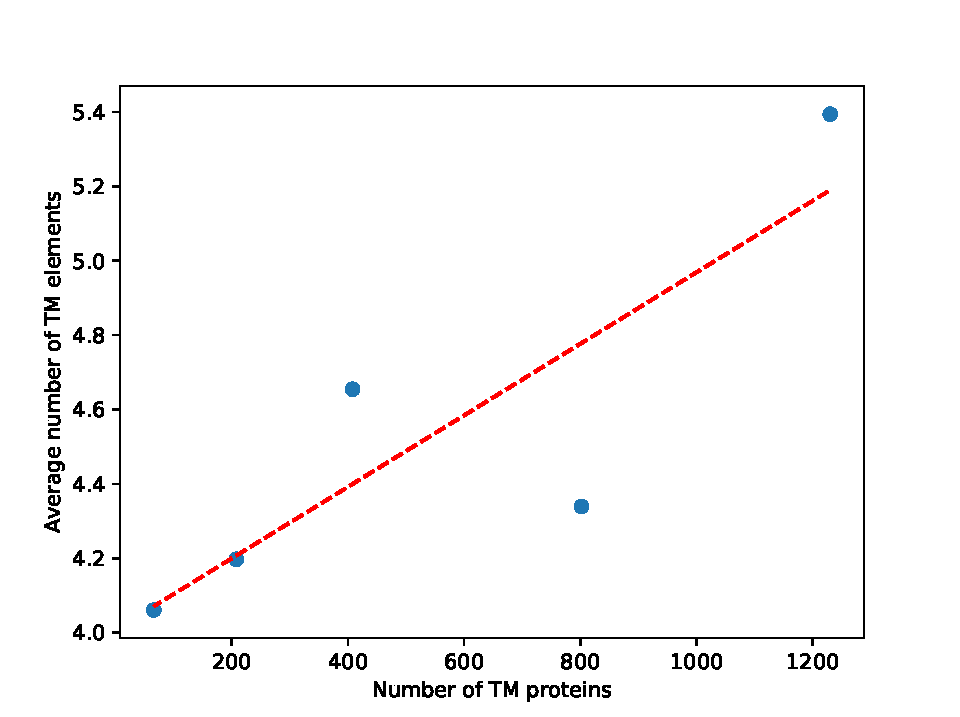
\includegraphics[width=1\textwidth]{Plot}
    \caption{Number of TM proteins vs TM segments}
    \label{fig:se}
\end{figure}


\end{document}
